\documentclass{beamer}
\usepackage{hyperref}
\usepackage{tipa}
%\usepackage[utf8]{inputenc}
\usepackage[space]{xeCJK}
\usepackage[T1]{fontenc}
\usepackage{verbatim}
\hypersetup{
    colorlinks=true,
    linkcolor=blue,
    filecolor=magenta,      
    urlcolor=blue,
}

\title{Hands on annotating data\\ with Praat}
\date{September 5, 2019}
\author{Rob van Son <\texttt{r.v.son@nki.nl}>}

\usetheme{Tapas}

\setbeamertemplate{footline}{\color{gray}
\hskip2cm    \parbox{\linewidth}{\vspace*{-15pt}\today \hskip2.5cm Annotating with Praat \hskip4cm\insertpagenumber}
}

%
%   This template is for PhD students from the TAPAS program
%
\begin{document}
% Don't modify this frame /!\ (frame title)
\begin{frame}[plain]
\titlepage
\end{frame}


%==================================================
% You can modify things here
\begin{frame} 
\frametitle{Introduction} 
\begin{block}{Annotating, segmenting, labelling}
\begin{itemize} 
\item Annotating\\ adding descriptive or analytic notations to language data
\item Segmenting\\ adding boundaries between ``elements'' in a recording
\item Labeling\\ adding annotations from a (fixed) lexicon
\item Transcripting/transliterating\\ converting sound into text
\item Example: Phonetic segmentation
\end{itemize}
\end{block} 
Rule: \textit{Never change the original recording or document}

\vskip 0.5cm
\scriptsize{For more information see:\\ P. Machač, R. Skarnitzl
 \textit{\href{https://www.researchgate.net/publication/234052076_Principles_of_Phonetic_Segmentation}{Principles of phonetic segmentation}}. Albatros Media a.s., 2012}
\end{frame}


\begin{frame} 
\frametitle{Praat} 
\begin{block}{Praat: doing phonetics by computer \hskip 0.5cm \url{www.praat.org}}
Praat is a computer program for analysing, synthesizing and manipulating speech and other sounds, and for creating publication-quality graphics.$^*$
\end{block} 
\begin{itemize} 
\item Visualizing speech and sounds
\item Analysis
\item Annotation
\item Manipulation
\item[$\Rightarrow$] Select \texttt{Help} when you are lost
\end{itemize}

\vskip 0.3cm
\scriptsize{$^*$\textit{The use of Praat in corpus research}.
In Jacques Durand, Ulrike Gut \& Gjert Kristoffersen (eds.): The Oxford handbook of corpus phonology, 342-360. Oxford: Oxford University Press, 2014.}
\end{frame}

\begin{frame} 
\frametitle{Preliminaries} 
\begin{block}{Recording and Metadata}
Published recordings made available at \href{https://datashare.is.ed.ac.uk/handle/10283/387}{datashare.is.ed.ac.uk}:

\textit{These sound recordings come from a wide range of participants, both male and female, during the 1950s and 60s, and are spoken in a variety range of languages.}
\end{block} 
\begin{itemize} 
\item Start \textit{Praat} from \href{http://www.praat.org}{praat.org}
\item \textit{The North Wind and the Sun}: recording \texttt{NW084.wav}
\item Text in Readme file
\item Recording \textit{NW084} contains name of speaker
\item \texttt{Praat > Open > Read from file...} open \texttt{NW084.wav}
\item \texttt{Praat > View \& Edit}
\end{itemize}
\end{frame}

\begin{frame} 
\frametitle{Navigating the \textit{Editor} window} 

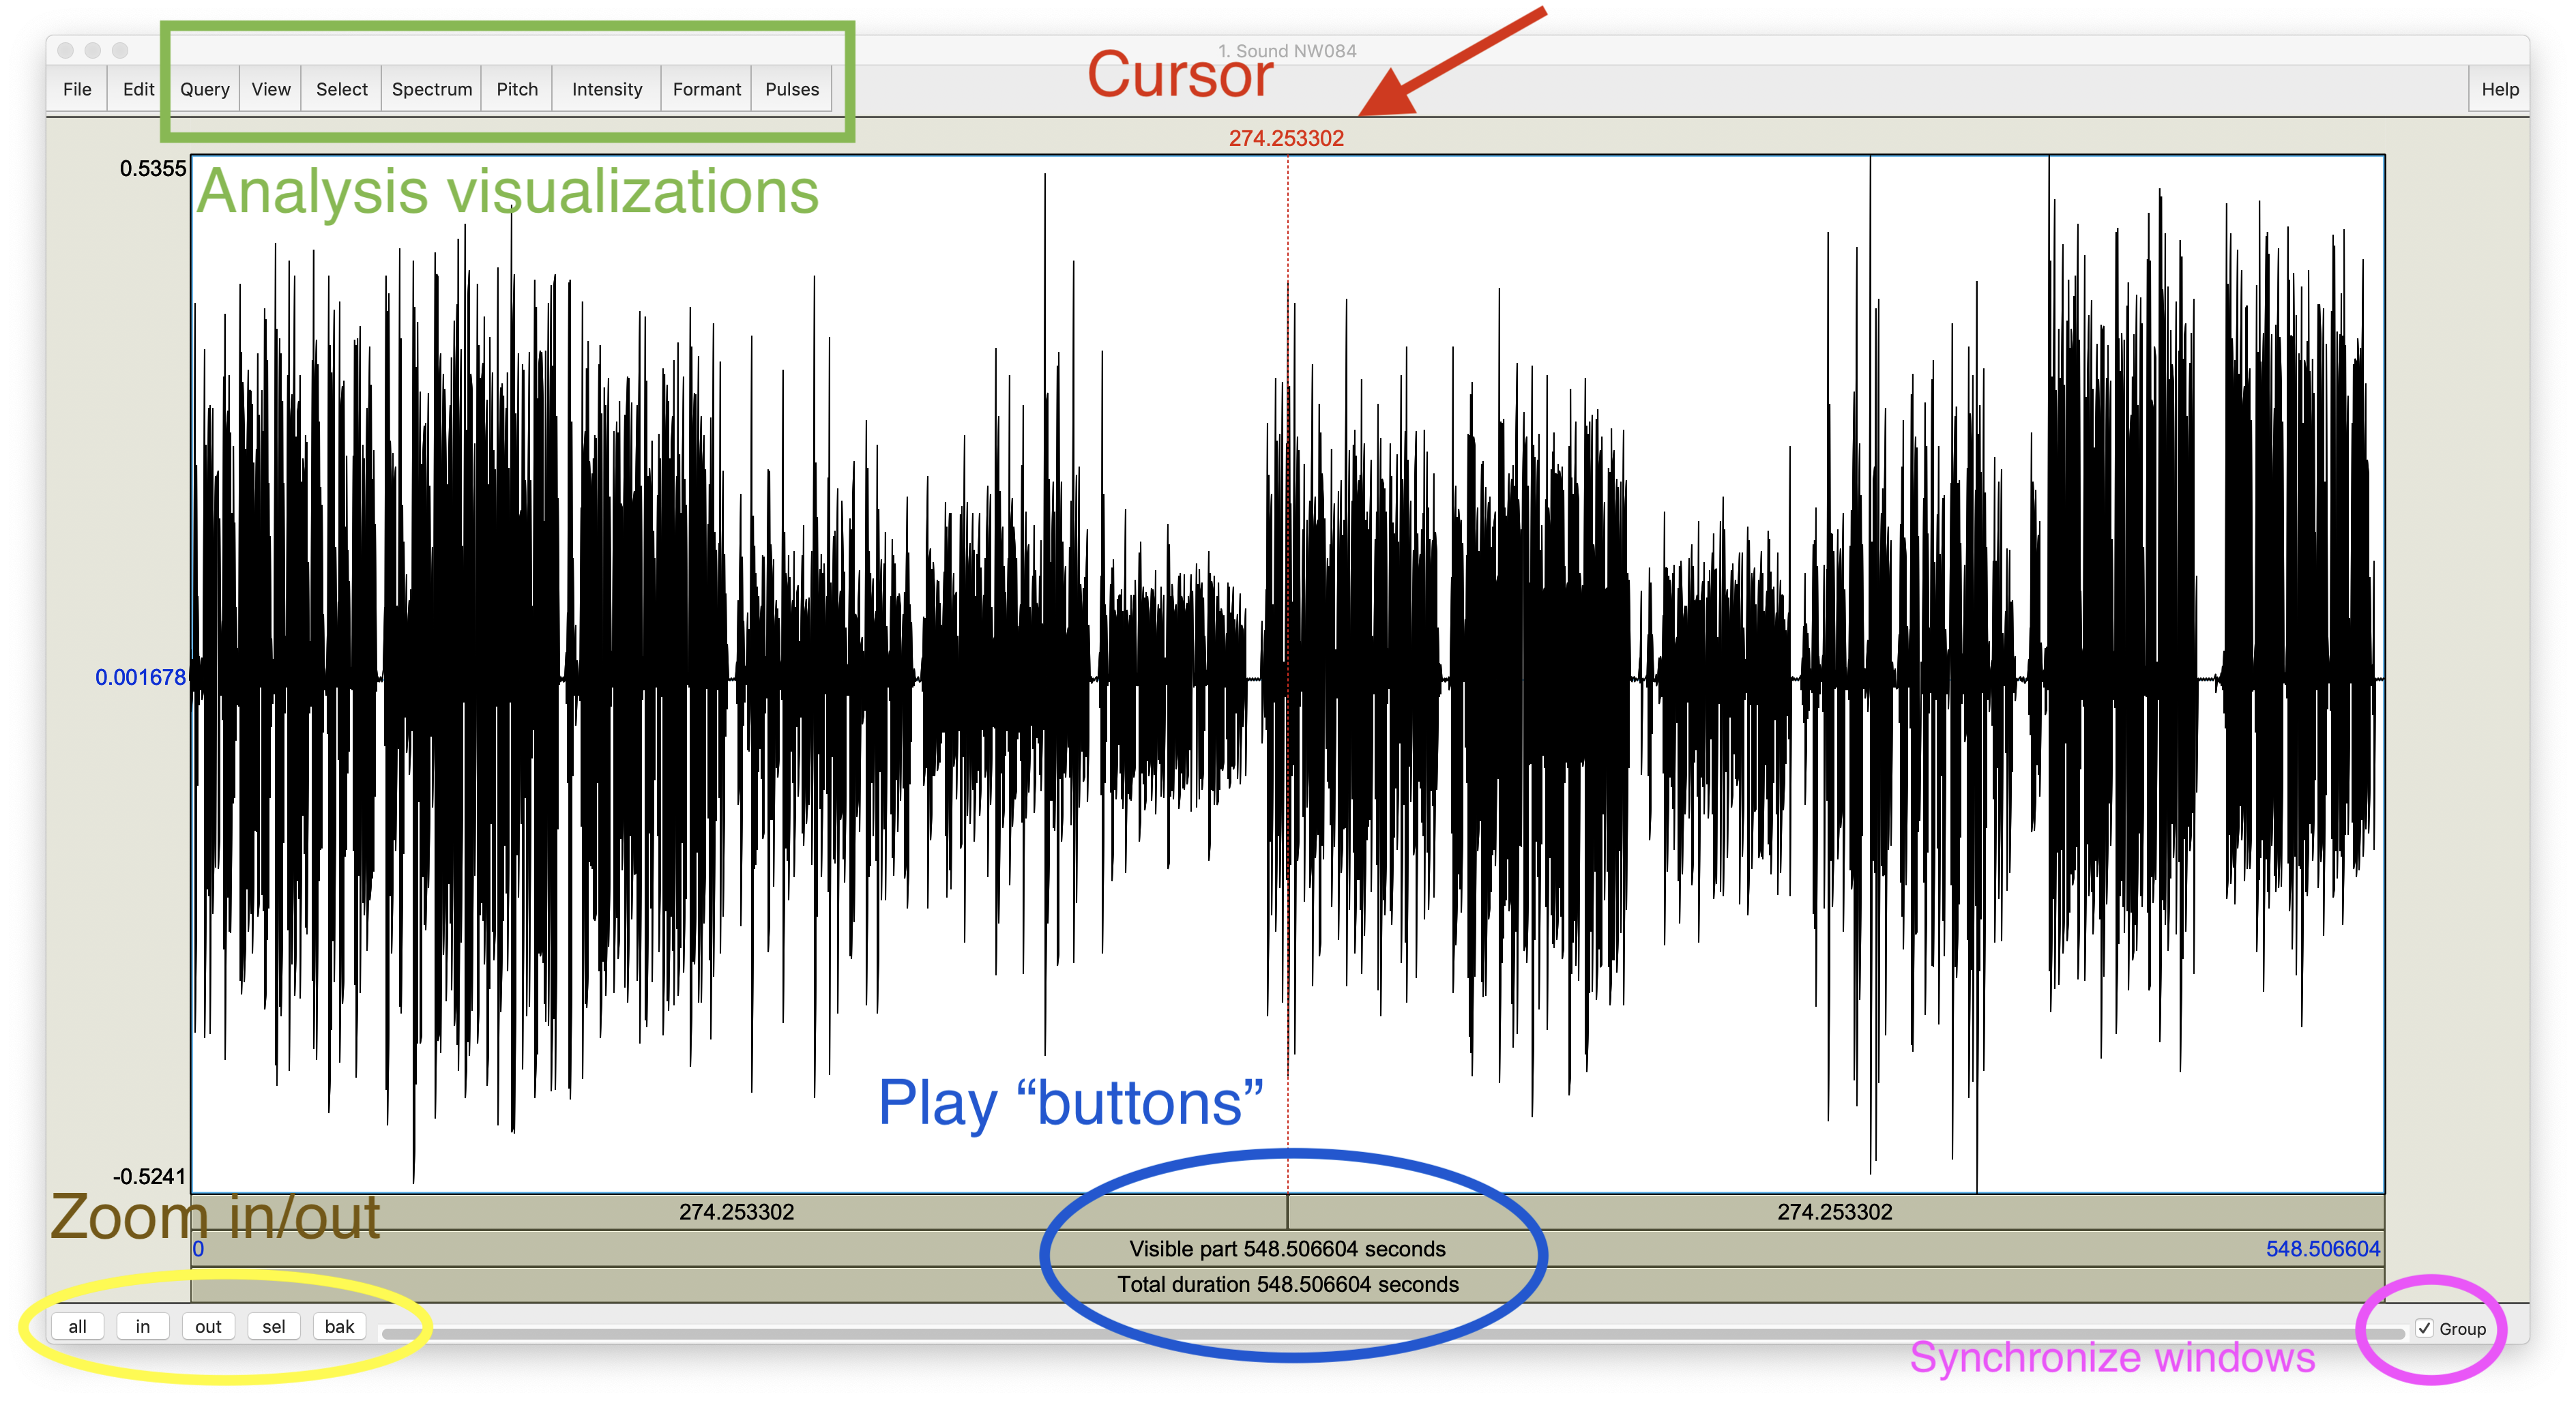
\includegraphics[width=1\framewidth]{img/Editor_Screenshot}

\end{frame}

\begin{frame} 
\frametitle{TextGrids} 
\begin{block}{Create and edit TextGrids}
\begin{itemize} 
\item Select Object: \texttt{Sound NW084}
\item \texttt{Praat > Annotate > To TextGrid...} 
\item In pop-up window set:
\begin{itemize} 
\item All tier names: \texttt{Sentences}
\item Which of these are point tiers?: Leave empty
\end{itemize}
\item Select both objects > View \& Edit
\item [ ]
\item To save your TextGrid
\begin{itemize} 
\item Select the TextGrid object
\item \texttt{Praat > Save > Save as short text file...}
\item Enter the name: \texttt{NW084.TextGrid} (preferably)
\item Click \texttt{Save}
\end{itemize}
\end{itemize}
\end{block} 
\end{frame}

\begin{frame} 
\frametitle{TextGrid Editor window} 

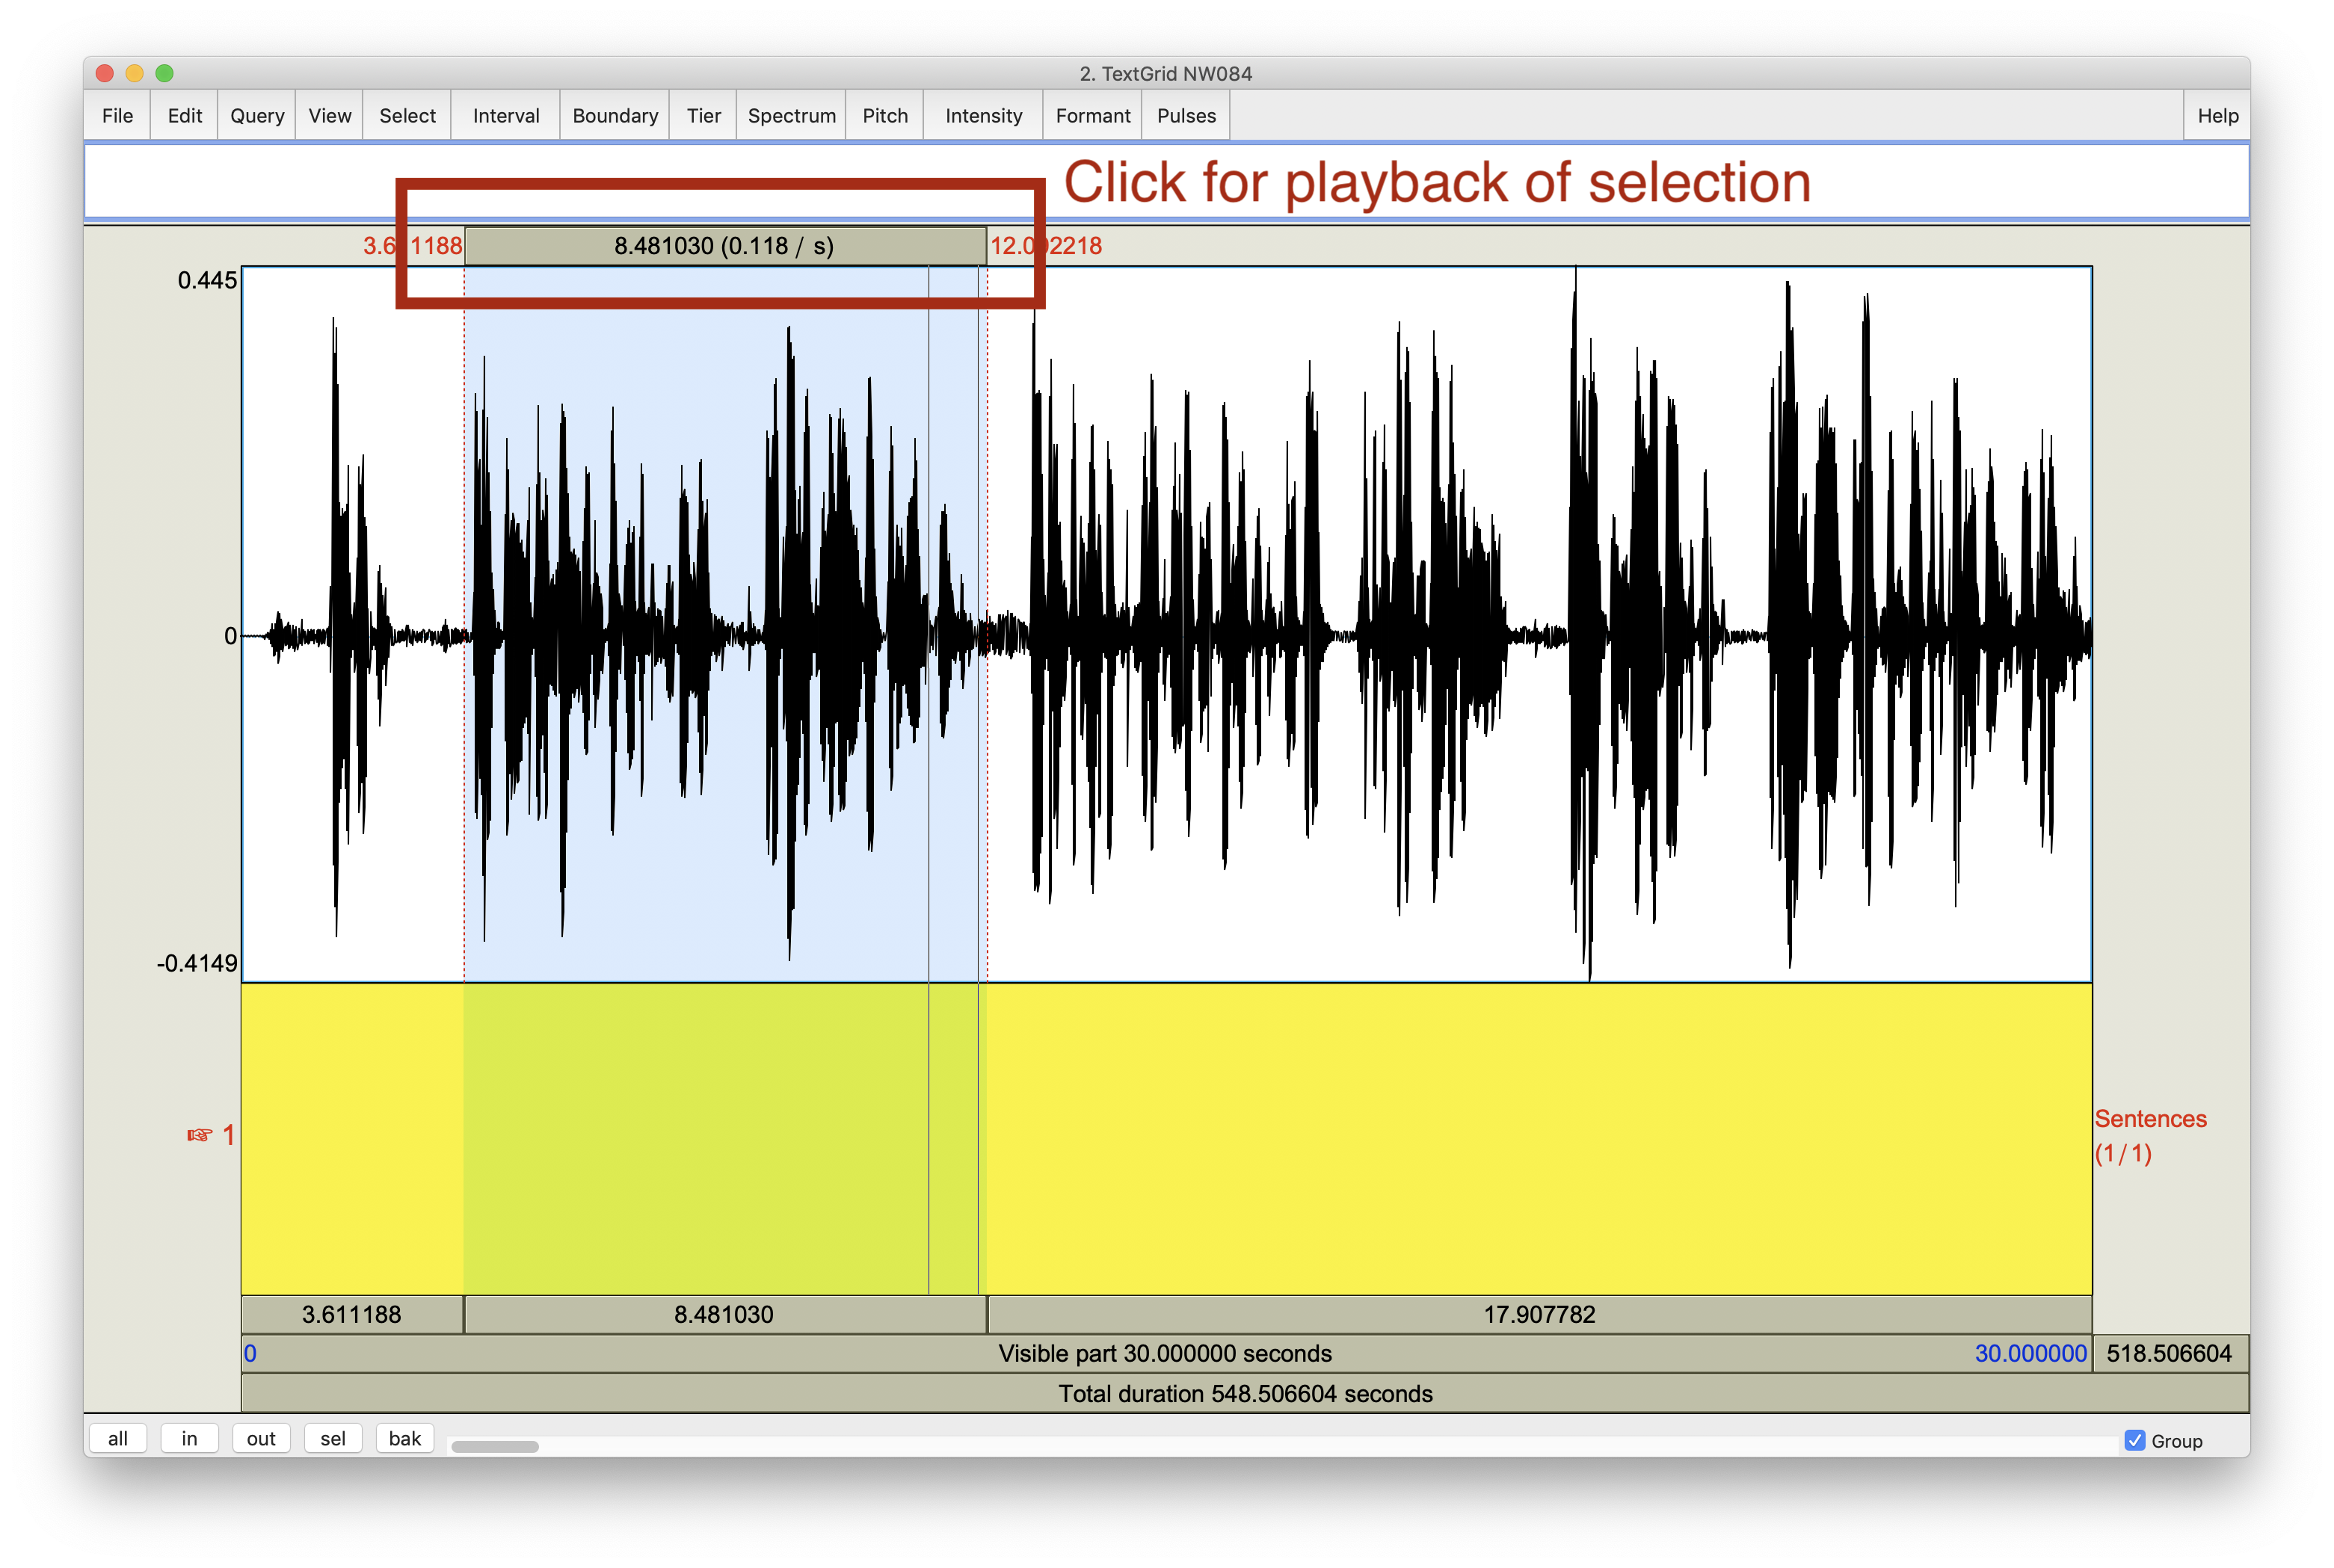
\includegraphics[width=0.71\framewidth]{img/Screenshot_TextGrid}
\vspace{-0.5cm}
\begin{itemize}
\item Use the cursor to select the first sentence:\\
      {\scriptsize{The North Wind and the Sun were disputing which was the stronger, when a traveller came along wrapped in a warm cloak}}
\item Listen to the selection by pressing the top bar
\item Press \texttt{Return} when you are done
\end{itemize}

\end{frame}

\begin{frame} 
\frametitle{TextGrid Editor window} 

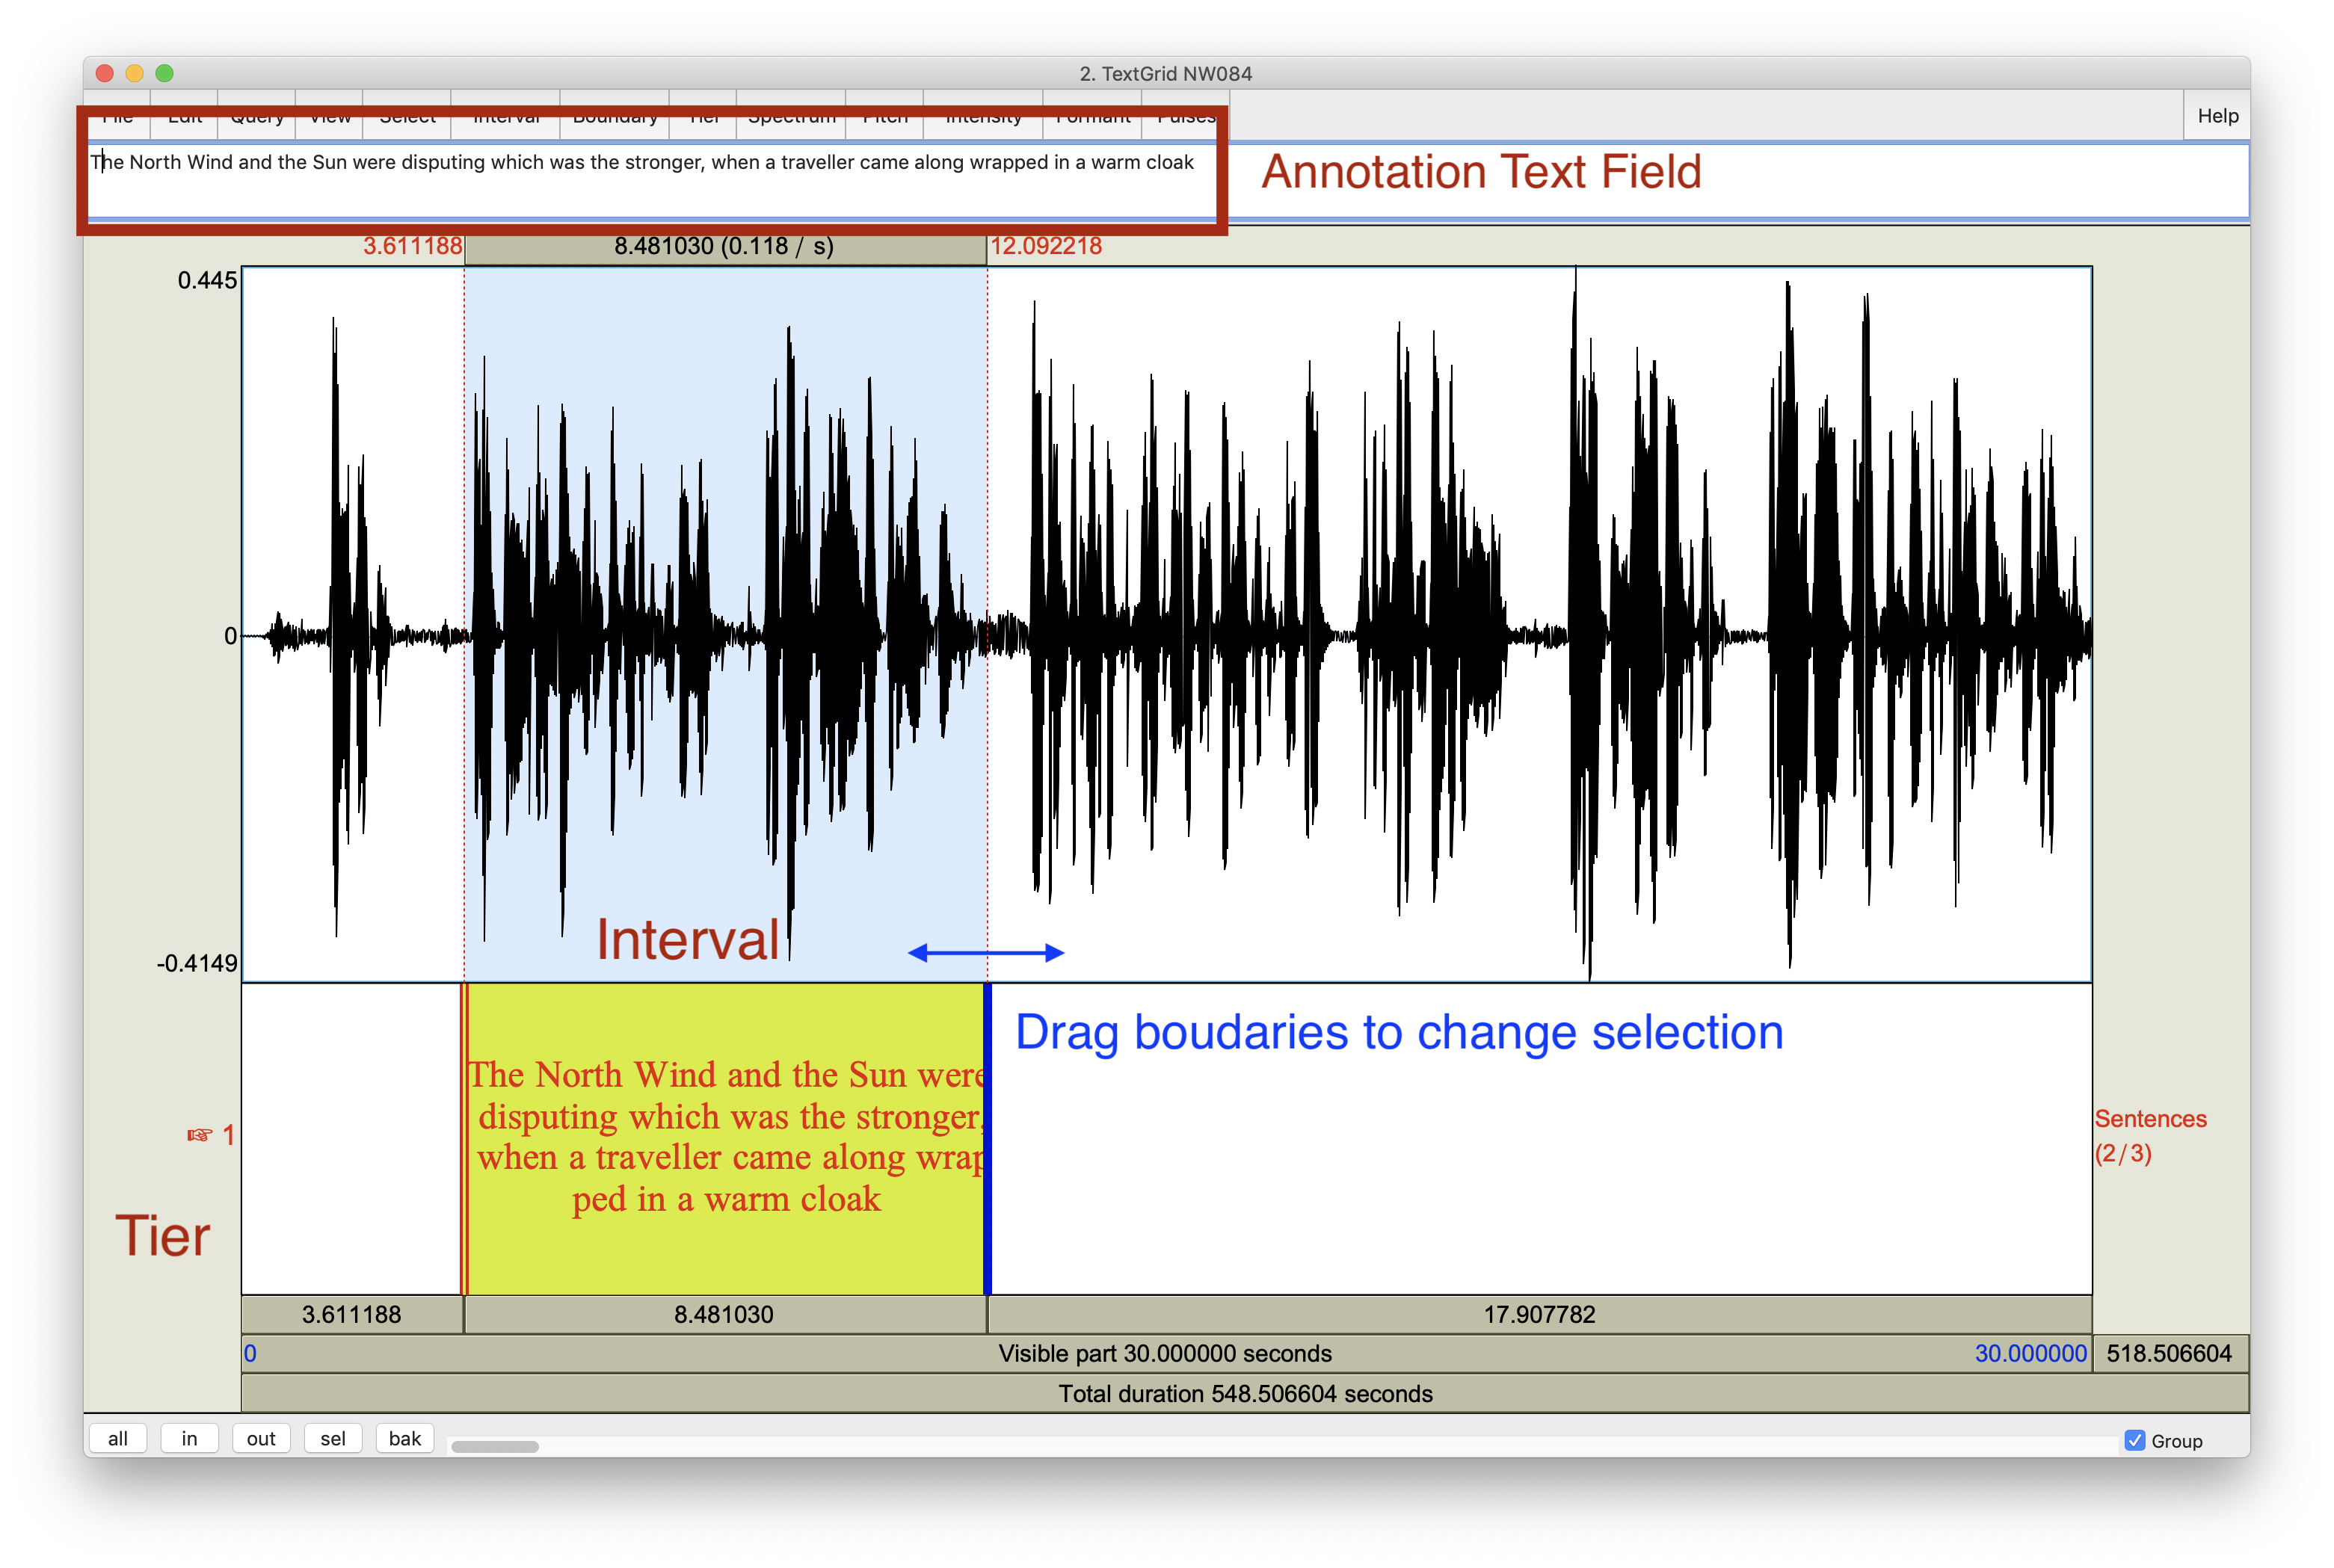
\includegraphics[width=0.71\framewidth]{img/Screenshot_Sentenses}
\vspace{-0.5cm}
\begin{itemize}
\item Enter the text into the top, annotation, field:\\
      {\scriptsize{The North Wind and the Sun were disputing which was the stronger, when a traveller came along wrapped in a warm cloak}}
\item Click on the interval when you are done
\item Do the same for the other sentences
\end{itemize}

\end{frame}

\begin{frame} 
\frametitle{Word segmentation} 
\begin{block}{Now segment and label the words}
Segment words in \textit{The North Wind and the Sun were disputing which was the stronger}
\end{block} 
\begin{itemize} 
\item Select Sentences Tier
\item \texttt{Editor > Tier > Duplicate tier...} \\Position: \texttt{1}, Name: \texttt{Words}
\item Select first sentence interval, click \texttt{sel} (bottom left)
\item \texttt{Editor > Spectrum > Show spectrogram}
\item Add a boundary between \textit{The} and \textit{North} \\(use cursor and click on circle)
\item Zoom in as far as needed
\item Add boundaries for the other words in the first phrase 
\end{itemize}
\end{frame}

\begin{frame} 
\frametitle{Segment \textit{The North wind}} 

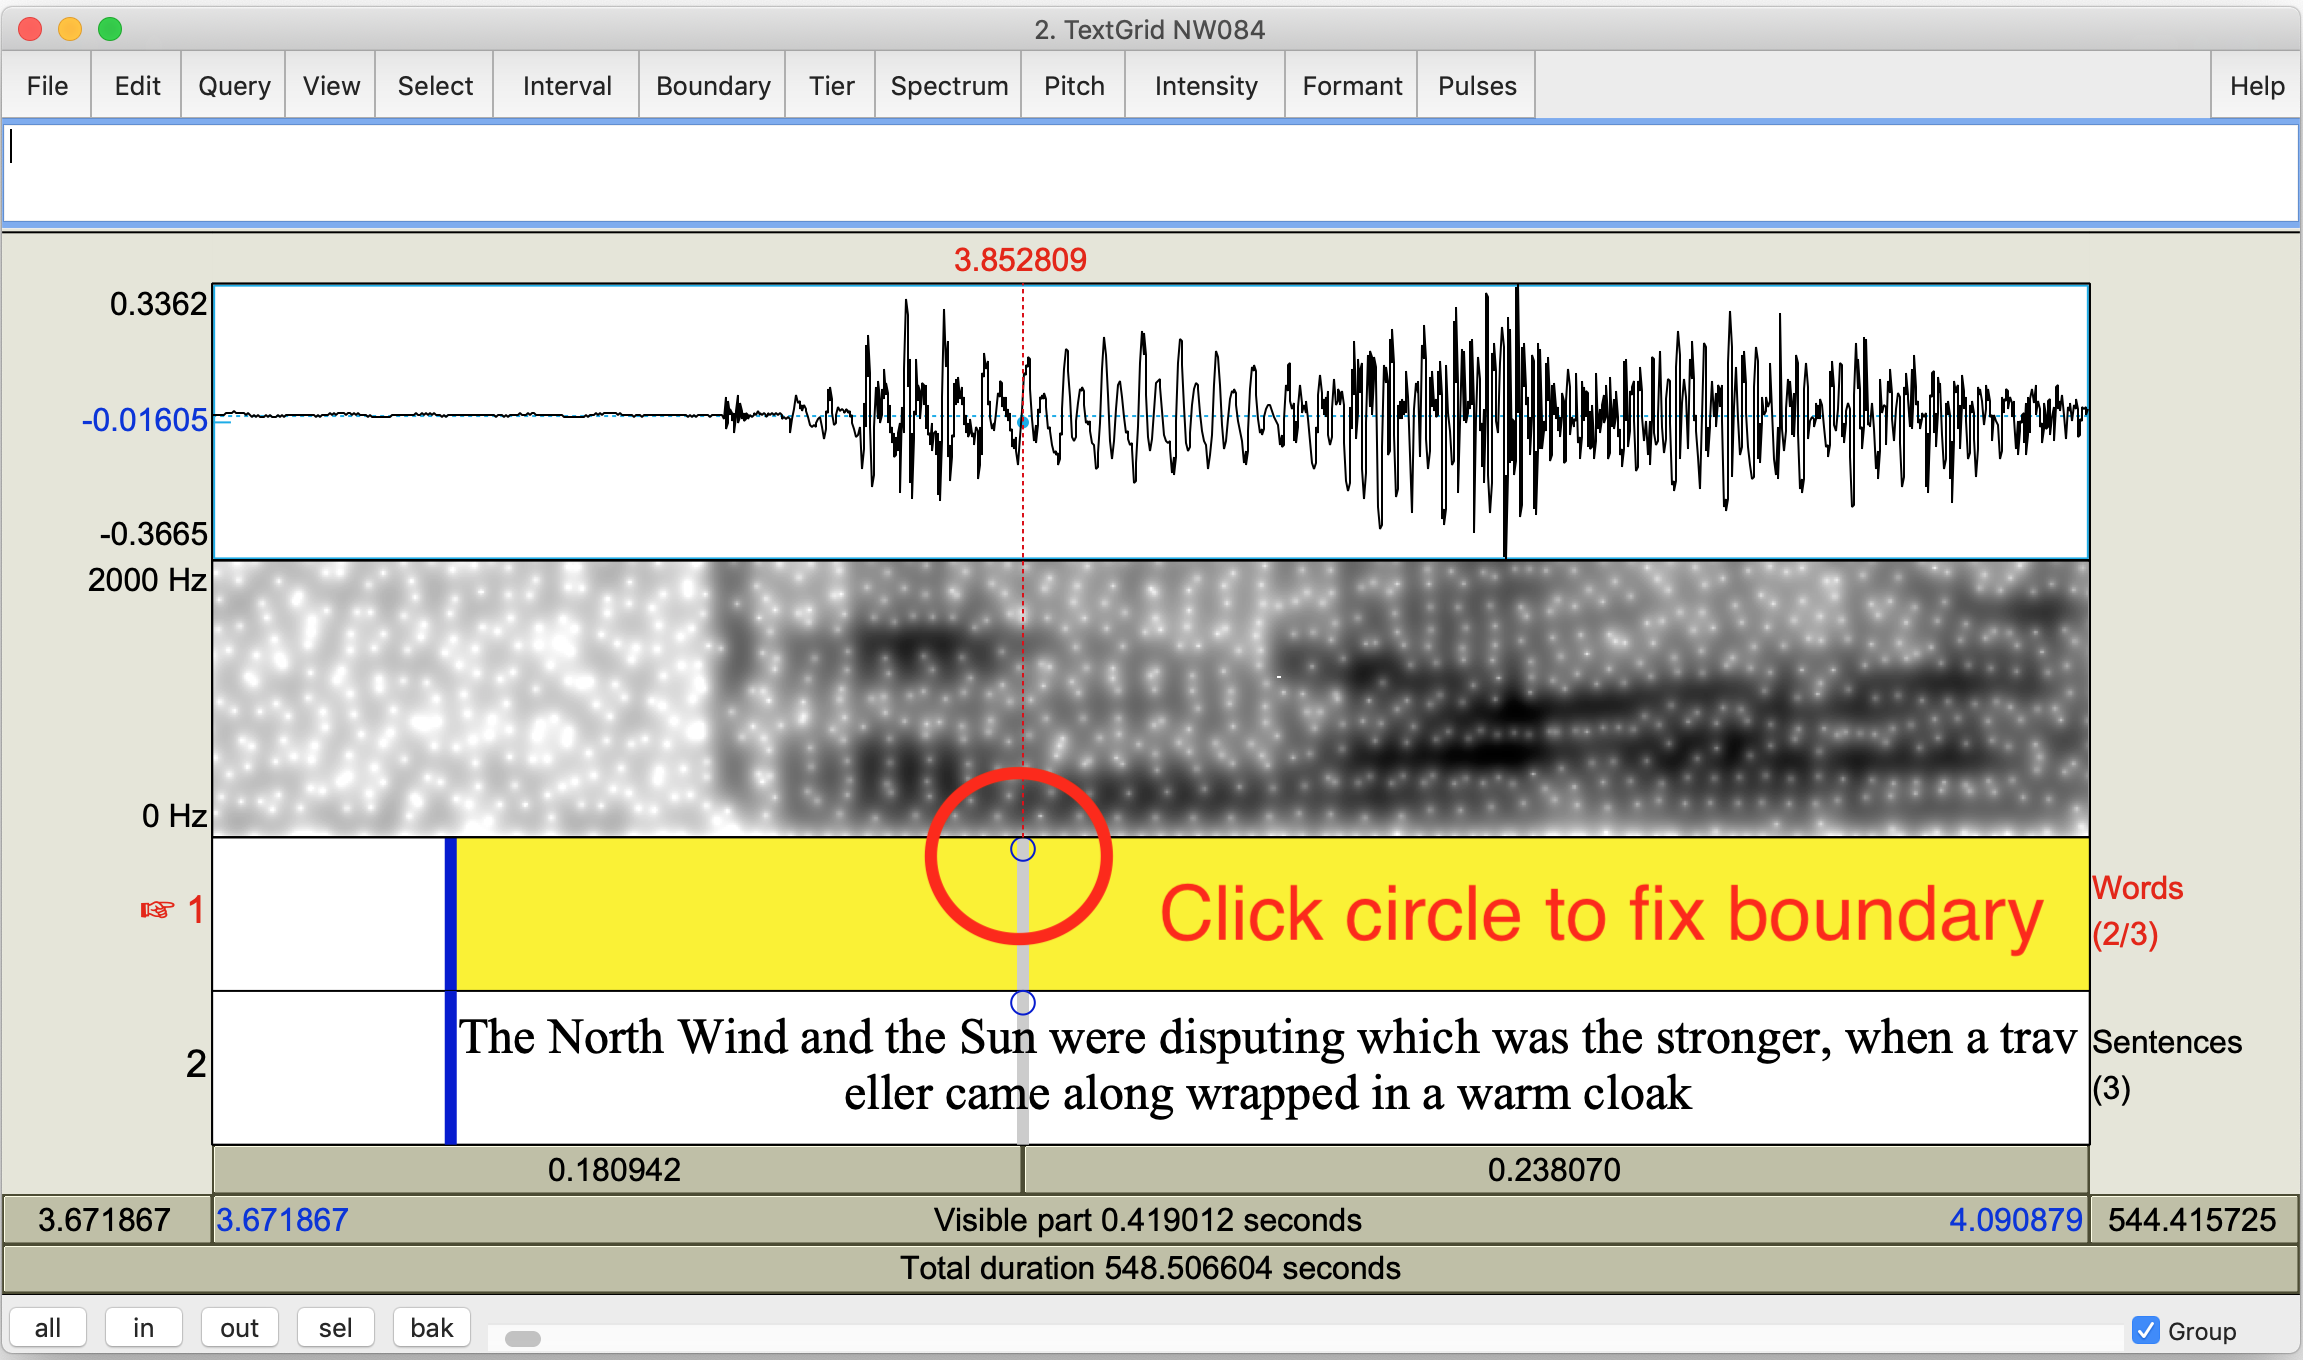
\includegraphics[width=0.95\framewidth]{img/Words_adding_boundary}

\begin{itemize} 
\item Listen to the fragments and look at the spectrogram
\item Add boundaries around \& between the first three words
\end{itemize}
\end{frame}

\begin{frame} 
\frametitle{Segment \textit{The North wind}} 

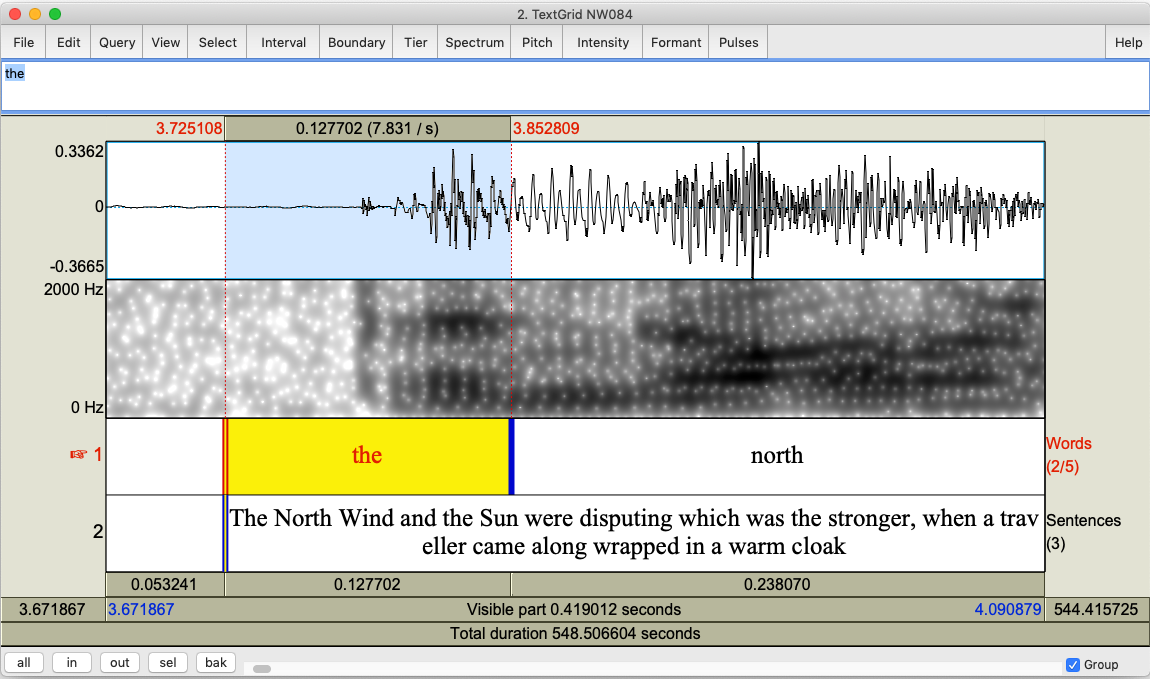
\includegraphics[width=0.95\framewidth]{img/Words_segmenting}

\begin{itemize} 
\item Add the words | \textit{the} | \textit{north} | \textit{wind} |
\item[ ]
\end{itemize}
\end{frame}

\begin{frame} 
\frametitle{Phonetic transcription} 
\begin{block}{Create phonetic transcription}
\begin{itemize}
\item Copy \textit{Words} tier to \textit{SAMPA} tier\\
\texttt{Editor > Tier > Duplicate tier...} \\Position: \texttt{1}, Name: \texttt{SAMPA}
\item Replace all words with their SAMPA$^*$ transcription\\ Use: \textit{North\_Wind\_and\_the\_Sun\_IPA\_SAMPA.txt}
\item Copy \textit{SAMPA} tier to \textit{Phonemes} tier\\
      \texttt{Editor > Tier > Duplicate tier...} \\Position: \texttt{1}, Name: \texttt{Phonemes}
\item Segment individual phonemes of \textit{The North wind}
\item Add SAMPA symbols
\end{itemize}
\end{block} 

\scriptsize{$^*$\url{https://www.phon.ucl.ac.uk/home/sampa/english.htm}}
\end{frame}

\begin{frame} 
\frametitle{Segment \textit{The North wind}} 

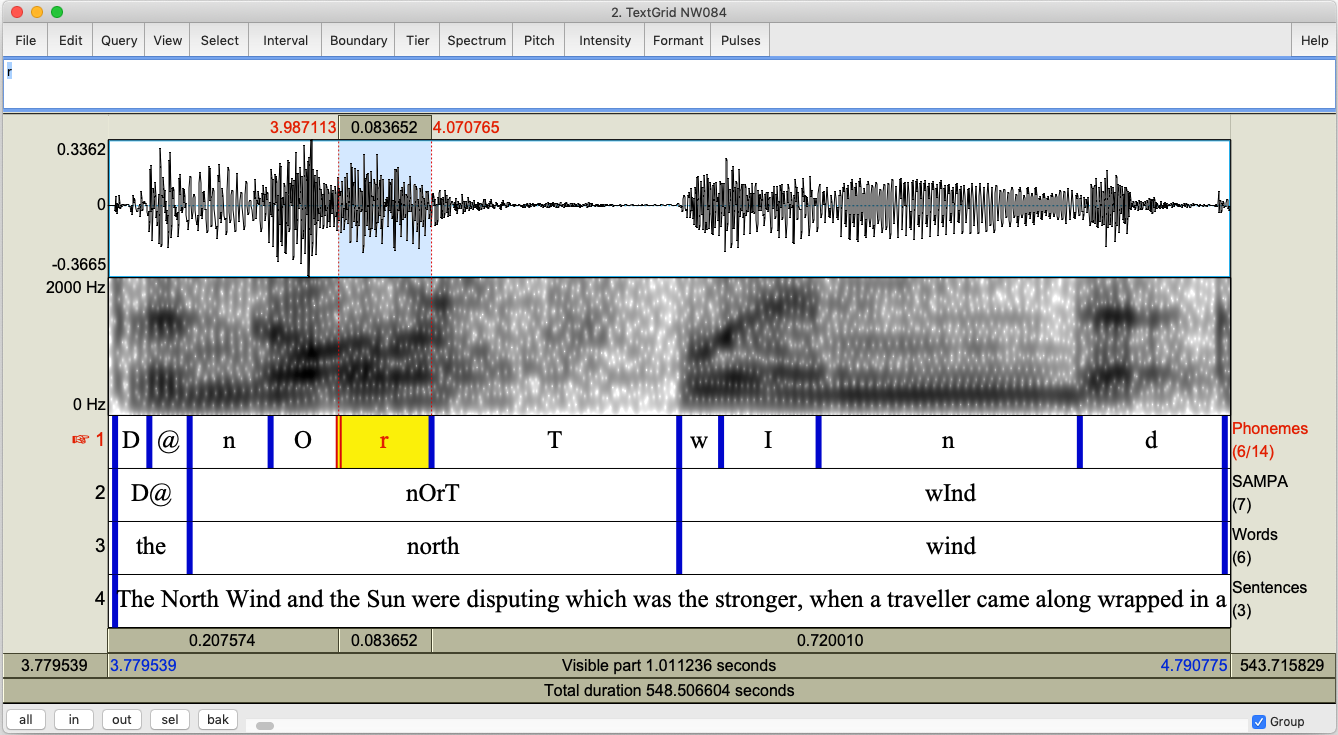
\includegraphics[width=0.95\framewidth]{img/Phonemes_segmentation}

\begin{itemize}
\item Add the boundaries
\item Add the phoneme labels (SAMPA)
\end{itemize}
\end{frame}

\begin{frame} 
\frametitle{Phonetic segmentation} 
\begin{block}{Tips and tricks (and traps)}
\begin{itemize} 
\item People do not always pronounce what you expect
\item Listen to whole words/phrases \\
      \textit{phonemes sound different in isolation than in context}
\item Phonemes are not beads on a string, they overlap
\item The ``best'' place to put a boundary is where it
\begin{enumerate}
\item separates the sounds as well as possible
\item marks a change in waveform \textbf{and/or} spectrogram
\end{enumerate} 
\item Boundaries do not always make sense
\begin{itemize} 
      \item[$\Rightarrow$] diphthongs and triphthongs are single phonemes \\
      (``I'': /\textipa{Ai}/, 秒 ``mi\v{a}o'': /\textipa{iau}/)
      \item[$\Rightarrow$] word-final /\textipa{@r}/ is often realized as /\textrhookschwa/
      \item[$\Rightarrow$] phonemes can be inseparable
\end{itemize}
\end{itemize}
\end{block} 
\end{frame}

\begin{frame} 
\frametitle{More annotations} 
\begin{block}{What else can be annotated? (non-exhaustive list)}
\begin{itemize} 
\item Non-verbal sounds:
\begin{itemize}
\item laughs, giggles
\item disturbances, coughing, other noises
\item conversation backchannels: \textit{hm},  \textit{uhm}, \textit{ok}
\end{itemize}
\item Speaker turns
\item Emotions, eye contact, smiles (with video$^*$)
\item Gestures and signs  (with video$^*$)
\item Focus and stress
\item Dialect \& Code switching
\end{itemize}
\end{block} 
In short: Anything that requires human interpretation

\vskip 0.5cm
$^*$\scriptsize{For video, you can use \href{https://tla.mpi.nl/tools/tla-tools/elan/}{ELAN} from: Max Planck Institute for Psycholinguistics, The Language Archive, Nijmegen, The Netherlands}

\end{frame}

\begin{frame} [fragile]
\frametitle{What to do with annotations? Praat Scripts} 
\vskip -0.5cm
\begin{block}{Scan all TextGrids in folder and print durations}
\begin{tiny}
\begin{verbatim}
writeInfoLine: "File", tab$, "Label", tab$, "Duration"
textGridList = Create Strings as file list: "List", "*.TextGrid"
numFiles = Get number of strings
for i to numFiles
    selectObject: textGridList
    textGridName$ = Get string: i
    currentTextGrid = Read from file: textGridName$
    numIntervals = Get number of intervals: 1
    for j to numIntervals
        label$ = Get label of interval: 1, j
        startTime = Get start time of interval: 1, j
        endTime = Get end time of interval: 1, j
        appendInfoLine: textGridName$, tab$, label$, tab$, 
...         fixed$(endTime - startTime, 3) 
    endfor
    selectObject: currentTextGrid
    Remove
endfor
selectObject: textGridList
Remove
\end{verbatim}
\end{tiny}

\end{block}
\textit{Duration} can be replaced by other measurements or actions
\vskip 0.2cm
\scriptsize{For more information see: \textit{\href{http://www.fon.hum.uva.nl/david/LOT/sspbook.pdf}{Speech Signal Processing with Praat}}
by David Weenink}
\end{frame}

\begin{frame} 
\frametitle{Scripting Praat} 
\begin{block}{Run a Praat script (e.g., \textit{TE3\_Example.praat})}
\begin{itemize} 
\item \texttt{Praat > Open Praat script...} Select script \\
      (Or: \texttt{Praat > Open > Read from file...} Select script)
\item \texttt{Editor > Run > Run}
\end{itemize}
\end{block} 

\begin{block}{My first Praat script}
\begin{itemize} 
\item Do once what you would like to code in \textit{Praat}
\item \texttt{Praat > New Praat script}
\item \texttt{Editor > Edit > Paste history}
\item Adapt script
\item \texttt{Praat > Help > Search Praat manual...} \textit{Scripting}
\end{itemize}
\end{block} 
\end{frame}

% Spare frame
\begin{frame} 
\frametitle{And then: Corpus construction} 
\begin{block}{Beyond audio and annotations}
\begin{itemize} 
\item Legal documentation:\\ Ethical board, informed consents, copyright transfers
\item Documentation and meta-data
\item Protocols for Recording and annotation
\item Storage \& distribution
\item Access \& licensing
\item Any programs and scripts used
\end{itemize}
\end{block} 
\vskip 1cm
See: \href{http://www.fon.hum.uva.nl/rob/NotesOnCorpora/NotesOnCorpusConstruction.pdf}{Notes on Corpus Construction}
\end{frame}


%==================================================
% keep this frame /!\ (Social media frame)
\begin{frame}
\frametitle{Social Media}
\small
\begin{tabular}{ll}
\hspace{-0.1cm}
\includegraphics[scale=0.4]{img/website.png} & \url{https://www.tapas-etn-eu.org}\vspace{0.3cm}\\ 

\includegraphics{img/twitter.png} & @TAPAS\_H2020\_ITN\vspace{0.4cm}\\

\includegraphics{img/facebook.png} & \url{https://www.facebook.com/TAPAS-H2020-MSCA-ITN-ETN}
\end{tabular}
\end{frame}

% Spare frame
\begin{frame} 
\frametitle{...} 
\begin{block}{...}
...
\end{block} 
\begin{itemize} 
\item ...
\end{itemize}
\end{frame}

\end{document}
